\documentclass[letterpaper,10pt]{article}
\usepackage{amsmath}
\usepackage{epsf, subfigure, verbatim, epsfig}
\usepackage{fancyhdr}
\usepackage{geometry}
\usepackage{calc}
\usepackage{ifthen}
\usepackage{layout}
\usepackage{fancybox}
\usepackage{eurosym}
\usepackage{tabularx}
\usepackage{xspace}
\usepackage{dsfont,mathrsfs}
\usepackage{amssymb}
\usepackage{theorem}
\usepackage{multicol}
\usepackage{float}

\pagestyle{fancy}

\topmargin-0.5in

\oddsidemargin-0.2in
\evensidemargin-0.5in
\textwidth6.8in
\textheight9in

\headheight0.2in
\fancyhfoffset[R]{0in}

\newcommand{\Sum}[2]{\ensuremath{\sum\limits}_{#1}^{#2}}
\newcommand{\bvec}[1]{\ensuremath{\mathbf{#1}}}

\theorempreskipamount .5cm \theorempostskipamount .5cm
\theoremheaderfont{\bfseries}
\theorembodyfont{\normalfont}

\newtheorem{thm}{Theorem}
\newtheorem{df}{Definition}[section]
\newtheorem{ex}{Exercise}
\newtheorem{lm}{Lemma}%[section]
\newtheorem{exa}{Example}[section]
\newtheorem{cor}{Corollary}%[section]
\newtheorem{alg}{Algorithm}%[section]
\newtheorem{inv}{Investigation}
\newtheorem{proj}{Project}



\lhead{Cal Poly} \chead{} %\rhead{dpaquin@calpoly.edu}
\lfoot{MATH 476} \rfoot{Mathematical Finance}

\begin{document}







\setcounter{tocdepth}{2}



\begin{center}

\Large

%{\bf Dr. Dana Paquin}\\

%{\bf dpaquin@calpoly.edu}\\

{\bf MATH 476: Special Topics in Applied Mathematics\\Mathematical Finance}\\

{\bf California Polytechnic State University}\\

{\bf Department of Mathematics}

\end{center}

\bigskip

\hrule

\bigskip


\tableofcontents


\bigskip

\hrule

\bigskip

\newpage



\section{Introduction to Financial Derivatives}



\subsection{Financial Derivatives}


\begin{df}{\bf Financial Derivative}
A {\bf financial derivative} is a financial instrument that has a value determined by (or {\em derived from}) the value of other underlying variables (i.e. the price of something else).  A derivative involves two parties agreeing to a future transaction.
\end{df}

\begin{itemize}

\item The derivatives market is much larger than the stock market when measured in terms of value of underlying assets. 

\item The value of the assets underlying outstanding derivatives transactions is several times the world gross domestic product. 

\item As we shall see in this unit, derivatives can be used for hedging or speculation or arbitrage. They can transfer a wide range of risks in the economy from one entity to another.

\item Often, the variables underlying derivatives are the prices of traded assets.  

\item For example, a stock option is a derivative whose value is dependent on the price of a stock.

\item However, derivatives can be dependent on almost any variable.  Examples include the price of gold, the value of a foreign currency, the price of corn, and  the amount of snow falling at a certain ski resort.

\item In general, derivatives provide an alternative to a simple sale or purchase, and thus increase the range of possibilities for an investor or manager seeking to accomplish some goal.  Derivatives are traded for a variety of reasons:

\begin{itemize}

\item {\bf Risk management}

\item {\bf Hedging}

\item {\bf Speculation}

\item {\bf Reduced transaction costs}

\item {\bf Regulatory arbitrage}

\end{itemize}

\item It is generally possible to create a given payoff in multiple ways. The construction of a given financial product from other products is called {\bf financial engineering}.

\item In recent years, and especially following the 2008 financial crisis, there have been many significant developments in the derivatives market.

\begin{itemize}

\item Many new instruments such as credit derivatives, electricity derivatives, weather derivatives, and insurance derivatives have been developed.

\item Many new types of interest rate, foreign exchange, and equity derivatives now trade.

\item There have been many new ideas in risk management and risk measurement.

\item Many regulations affecting the over-the-counter derivatives market have been introduced.

\item The {\em risk-free} discount rate used to value derivatives has changed and the decision has been taken to phase out LIBOR.

\item Derivatives dealers now adjust the way they price derivatives to allow for credit risks, funding costs, and capital requirements.

\item Collateral and credit issues are now given much more attention and have led to changes in the way derivatives are traded.

\item Machine learning is now becoming widely used for managing derivatives portfolios.

\end{itemize}

\end{itemize}

\bigskip

\hrule

\bigskip

\subsection{Financial Markets}

The trading of a financial asset contains (at least) four discrete steps:

\begin{enumerate}

\item The buyer and seller must locate one another and agree on a price. Stock exchanges, derivatives exchanges, and dealers all facilitate trading, providing buyers and sellers a means to find one another.

\item Once the buyer and seller agree on a price, the trade must be {\em cleared}, i.e., the obligations of each party are specified. In the case of a stock transaction, the buyer will be required to deliver cash and the seller to deliver the stock. In the case of some
derivatives transactions, both parties must post collateral.

\item The trade must be settled, that is, the buyer and seller must deliver in the required period of time the cash or securities necessary to satisfy their obligations.

\item Once the trade is complete, records are updated.

\end{enumerate}

Trading of financial claims often takes place on organized {\bf exchanges}. 

\begin{df}{\bf Exchange}
An {\bf exchange} is an organization that provides a venue for trading, and that sets rules governing what is traded and how trading occurs. 
\end{df}

\begin{itemize}

\item A given exchange will trade a particular set of financial instruments.

\item The New York Stock Exchange (NYSE) is an example of an exchange.

\item The Chicago Board of Trade (CBOT) was established in 1848 to bring farmers and merchants together. Initially its main task was to standardize the quantities and qualities of the grains that were traded. Within a few years, the first futures-type contract was developed. It was known as a to-arrive contract. Speculators soon became interested in the contract and found trading the contract to be an attractive alternative to trading the grain itself.

\item The Chicago Board Options Exchange (CBOE, www.cboe.com) started trading call option contracts on 16 stocks in 1973. Options had traded prior to 1973, but the CBOE succeeded in creating an orderly market with well-defined contracts. Put option contracts started trading on the exchange in 1977. The CBOE now trades options on thousands of stocks and many different stock indices.

\item Traditionally derivatives exchanges have used what is known as the {\bf open outcry system}. This involves traders physically meeting on the floor of the exchange, shouting, and using a complicated set of hand signals to indicate the trades they would like to carry out. 

\item Exchanges have largely replaced the open outcry system by {\bf electronic trading}. This involves traders entering their desired trades at a keyboard and a computer being used to match buyers and sellers. 

\item Electronic trading has led to a growth in {\bf high-frequency trading}. This involves the use of algorithms to initiate trades, often without human intervention, and has become an important feature of derivatives markets.


\item After a trade has taken place, a {\bf clearinghouse} matches the buyers and sellers, keeping track of their obligations and payments. The traders who deal directly with a clearinghouse are called clearing members. If you buy a share of stock as an individual, your transaction ultimately is cleared through the account of a clearing member.

\item With stock and bond trades, after the trade has cleared and settled, the buyer and seller have no continuing obligations to one another. However, with derivatives trades, one party may have to pay another in the future. To facilitate these payments and to help manage credit risk, a derivatives clearinghouse typically interposes itself in the transaction, becoming the buyer to all sellers and the seller to all buyers. This substitution of one counterparty for another is known as {\bf novation}.


\end{itemize}

\begin{df}{\bf Over The Counter (OTC ) Markets}
It is possible for large traders to trade many financial claims directly with a dealer, bypassing organized exchanges. Such trading is said to occur in the {\bf over-the-counter (OTC) market}.
\end{df}

\begin{itemize}

\item Most of the trading volume numbers we see reported in the newspaper/online pertain to exchange-based trading. 

\item Exchange activity is public and highly regulated. Over-the-counter trading is not easy to observe or measure and is generally less regulated. 

\item For many categories of financial claims, the value of OTC trading is greater than the value traded on exchanges.

\item The number of derivatives transactions per year in OTC markets is smaller than in exchange- traded markets, but the average size of the transactions is much greater. 

\item Although the statistics that are collected for the two markets are not exactly comparable, it is clear that the volume of business in the over-the-counter market is much larger than in the exchange-traded market. 

\end{itemize}


\begin{figure}[ht]
\begin{center}
\includegraphics[scale=0.5]{markets.png}
\caption{Size of over-the-counter and exchange-traded derivatives markets.}
\end{center}
\end{figure}


\bigskip

\hrule

\bigskip

\subsection{Buying and Short-Selling Financial Assets}

\begin{df}{\bf Ask Price}
The price at which you can buy a financial asset is called the {\bf offer price} or {\bf ask price}.
\end{df}

\begin{df}{\bf Bid Price}
The price at which you can sell a financial asset is called the {\bf bid price}.
\end{df}

\begin{df}{\bf Bid-Ask Spread}
The difference between the price at which you can buy and the price at which you can sell is called the {\bf bid-ask spread}.
\end{df}

\begin{df}{\bf Short Sale}
The sale of a financial derivative that you do not currently own is called a {\bf short sale}.  Short sales can be used for {\em speculation}, {\em financing}, or {\em hedging}.
\end{df}

\bigskip

\hrule

\bigskip

\subsection{Forwards and Futures}

\begin{df}{\bf Spot Contract}
A {\bf spot contract} is an agreement to buy or sell an asset (almost) immediately. 
\end{df}

\begin{df}{\bf Forward Contract}
A {\bf forward contract} is an agreement to buy or sell an asset at a certain future time for a certain price.  The {\em long position} (the purchaser of the forward contract) in the forward contract agrees to {\em buy} the asset on a specified future date for a specified price, and the {\em short position} (the seller of the forward contract) agrees to sell the asset on that date for the specified price.  Forwards contracts are traded in the over-the-counter market.
\end{df}

\begin{df}{\bf Futures Contract}
A {\bf futures contract} is an agreement between two parties to buy or sell an asset at a certain time in the future for a certain price. Futures contracts are normally traded on an exchange.
\end{df}

\noindent We use the following notation:

\begin{itemize}

\item $K=$ delivery price of the forward contract (the price at which the long position agrees to buy the asset)

\item $S_T=$ spot price of the asset at maturity of the contract (time $T$)

\end{itemize}

\begin{ex}{\bf Forward Contract Payoff}


\begin{itemize}

\item Find the payoff from a long position in a forward contract on one unit of an asset.

\item Find the payoff from a short position in a forward contract on one unit of an asset.

\end{itemize}


\end{ex}


\begin{ex}{\bf Forward Contract on Stock Index}
Suppose that the S\&R 500 index has a current price of \$1000, and the $6$-month forward price is \$1020.  What happens if the index price is \$950 in $6$ months?  \$1200 in $6$ months?  Construct payoff diagrams for the long and short positions on this contract.  What would be an advantage of using the forward contract to buy the index in $6$ months, as opposed to buying it outright at time $t=0$?  
\end{ex}


\begin{ex}{\bf Payoff Diagrams for Forward Contract}
Construct payoff diagrams for the long and short positions in a forward contract with delivery price $K$ and spot price $S_T$.
\end{ex}



\begin{ex}{\bf Forward Contract on Foreign Exchange}
Forward contracts on foreign exchange are very popular. Most large banks employ both spot and forward foreign-exchange traders.   The table below shows quotes for the exchange rate between the British pound (GBP) and the U.S. dollar (USD) in May 2020. The quote is for the number of USD per GBP.

\begin{center}
\begin{table}[h]
\begin{tabular}{|c|c|c|}\hline
&Bid&Ask\\\hline
Spot & 1.2217&1.2220\\\hline
$1$-month forward & 1.2218&1.2222\\\hline
$3$-month forward & 1.2220&1.2225\\\hline
$6$-month forward & 1.2224&1.2230\\\hline
\end{tabular}
\caption{Forward contract on foreign exchange USD per GBP, May 2020}
\end{table}
\end{center}

\noindent Suppose that the treasurer of a U.S. corporation knows that it will pay $1$ million GBP in $6$ months, and wants to hedge against exchange rate changes.  Suppose that the bank agrees to a $6$-month forward contract to purchase $1$ million GBP in $6$ months.  What happens if the spot exchange rate is 1.3000 in 6 months?  What if the spot exchange rate is 1.2000 in 6 months?

\end{ex}

\begin{ex}
An investor enters into a short forward contract to sell 100,000 British pounds for U.S. dollars at an exchange rate of 1.3000 USD per pound. How much does the investor gain or lose if the exchange rate at the end of the contract is (a) 1.2900 and (b) 1.3200?
\end{ex}


\begin{ex}
A trader enters into a short forward contract on 100 million yen. The forward exchange rate is \$0.0090 per yen. How much does the trader gain or lose if the exchange rate at the end of the contract is (a) \$0.0084 per yen and (b) \$0.0101 per yen?
\end{ex}

\newpage


\section{Introduction to Options}

\subsection{Call and Put Options}

\begin{df}{\bf European call option}
A {\bf European call option} is a contract that gives the holder the {\em right to buy} an {\em underlying asset} for a certain fixed price $K$, called the {\bf exercise price}, or {\bf strike price}, at a specified future time $T$, called the {\bf exercise time} or {\bf expiry time}. 
\end{df}

\begin{df}{\bf European put option}
A {\bf European put option} gives the holder the {\em right to sell} an underlying asset for the strike price $K$ at the exercise time $T$.
\end{df}

\begin{df}{\bf American call option}
An American call option gives the holder the right to buy the underlying asset at the strike price $K$ at any time {\em between} now and the expiry time $T$.
\end{df}

\begin{df}{\bf American put option}
An American put option gives the holder the right to sell the underlying asset at the strike price $K$ at any time {\em between} now and the expiry time $T$.
\end{df}

\noindent Our initial focus will be on European options.  It should be emphasized that an option gives the holder the {\em right} to do something; the holder does not have to exercise this right.  The other party involved, who is known as the {\em writer}, does have a potential obligation:  in the case of a call option, he {\em must} sell the asset if the holder chooses to buy it, and in the case of a put option, he must buy the asset if the holder chooses to sell it.  Since the option confers on its holder a right with no obligation, it has some value.  Moreover, it must be paid for at the time of opening the contract.  Conversely, the writer of the option most be compensated for the obligation he has assumed.  Two of our main areas of exploration throughout this section are:

\begin{itemize}

\item How much would one pay for this right, i.e. what is the value of an option?

\item How can the writer minimize the risk associated with this obligation?

\end{itemize}



\begin{ex}\label{call-ex}{\bf A Call Option}
Consider the following European call option.  Let $T$ denote the date exctly 10 days from now.  At time $T$, the holder of the option {\em may} purchase one share of XYZ stock for \$250.  To gain an understanding of how call options work and what might be reasonable for the price of this option, we will consider two possible situations that might occur on the expiry time $T$.  Let $S_T$ denote the price of one share of XYZ stock at time $T$.

\begin{itemize}

\item What happens if $S_T=\$270$?




\item What happens if $S_T=\$230$?


\end{itemize}

\end{ex}

\begin{ex}\label{expected-payoff}
Suppose that the XYZ share in example \ref{call-ex} only takes the values \$230 or \$270 with equal probability.  Find the expected payoff at time $T$ on the call option.  This expected value is a useful approximation for what a reasonable amount to pay for the call option would be.  
\end{ex}

\begin{ex}
Let $c$ denote the expected payofft that you obtained in Exercise \ref{expected-payoff}.  Although option pricing is, in general, more complicated, suppose that the holder of the option did pay \$c for this option.  
\begin{enumerate}
\item[(a)] What is his net profit or loss if $S_T=\$270$?  Express the net profit or loss in this case as a percentage of the initial cost of the option.

\item[(b)] What is his net profit or loss if $S_T=\$230$?  Express the net profit or loss in this case as a percentage of the initial cost of the option.
\end{enumerate}
\end{ex}

\begin{ex}
Suppose that, instead, the investor purchased the share for \$250 instead of purchasing the option.  Express his net profit or loss in each case (i.e. $S_T=\$230$ or $S_T=\$270$) as a percentage of the initial cost of purchasing the share.  Compare with the results of the previous exercise.
\end{ex}  

\begin{center} {\bf The key idea behind the results of the previous two exercises is that options respond in an exaggerated way to changes in the underlying asset price.}
\end{center}

\begin{itemize}

\item From this simple example, we see that the greater the share price at time $T$, the greater the profit.  However, we do not, of course, know that price in advance.  

\item However, it is reasonable to assume that the higher the share price is now (a quantity we {\em do} know) then the higher the price is likely to be in the future.  

\item Thus, the value of a call option {\em today} should depend on today's share price.  

\item Similarly, the value of the call option also depends on the exercise price:  the lower the exercise price, the less that has to be paid on exercise, and so the higher the option value.  

\item Observe that just before the option is to expire, there is little time for the asset price to change, so in that case, the price at expiry is known with a fair degree of certainty.  Thus, we can conclude that the price of the call option should also depend on the time to expiry.

\item Additionally, we will see that the option price depends on the ``randomness" of the stock price--this randomness is known as the {\em volatility}.  The larger the volatility, the more ``jagged" the graph of the stock price is as a function of time.  

\item Finally, the option price should depend on interest rates, as the option is paid for at the time of purchase (rather than at the time of expiry).  The payoff (if any) does not come until later (at expiry), so the option price should reflect the income that would otherwise have been earned by investing the premium (the cost of the option) in the bank and earning interest.  

\end{itemize}

Thus, we conclude in this introductory section that the price of an option should depend on (at least) the following:

\begin{itemize}

\item The current price of the stock, $S_0=S(0)$

\item The strike price, $K$

\item The time to expiration, $T$

\item The volatility of the stock price, $\sigma$

\item The interest rate, $r$

\end{itemize}



\begin{ex}{\bf A Put Option}
Consider an investor who buys a European put option to sell 100 shares of stock XYZ with a strike price of \$70.  Suppose that the current stock price is \$65.   What happens if $S_T=\$55$?



\end{ex}

\begin{ex}
It is important to observe that sometimes an investor chooses to exercise an option even though he may make a loss overall.  For example, suppose that an investor buys a European call option with a strike price of \$100 per share to buy 100 shares of XYS stock, and that the current stock price is \$98 per share.  The price of the option to purchase these 100 shares is \$500.  Suppose that the price of the stock is \$102 per share at expiry.  Explain why it is preferable for the investor to exercise the option in this case, even though he makes a loss overall.
\end{ex}






Note that there are two sides to every option contract.  On one side, there is the investor that has bought the option; this is called taking the {\em long position} in the option.  On the other side, there is the investor that has sold or written the option; this is called taking the {\em short position} in the option.  The investor in the short position receives cash up front (for selling the option), but has potential liabilities later.  

To summarize, there are four types of option positions:

\begin{enumerate}

\item A long position in a call option

\item A long position in a put option

\item A short position in a call option

\item A short position in a put option

\end{enumerate}

\bigskip

\hrule

\bigskip

\subsection{Option Payoffs}

It is often useful to characterize European option positions in terms of the terminal value or {\em payoff} to the investor at maturity.  The initial cost of the option is not included in this calculation.  Let $K$ denote the strike price and let $S_T$ denote the price of the stock at the expiry of the option.  

\begin{ex}{\bf Payoffs from Positions in European Call Options}
Find each of the following.
\begin{enumerate}
\item[(a)] The payoff to the holder of a long position in a European call option.

\item[(b)] The payoff to the holder of a short position in a European call option.



\item[(c)] The payoff to the holder of a long position in a European put option.


\item[(d)] The payoff to the holder of a short position in a European put option.


\end{enumerate}
\end{ex}

\begin{ex}{\bf Payoff Diagrams for Positions in European Call Options}
Construct payoff diagrams for each of the four positions above (long call, short call, long pout, short put).
\end{ex}



\begin{ex}
An investor buys a European put on a share for \$3.  The stock price is \$42, and the strike price is \$40.  Under what circumstances does the investor make a profit?  Under what circumstances will the option be exercised?  Draw a profit diagram illustrating the variation of the investor's {\em profit} (not the payoff) with the stock price at the maturity of the option.
\end{ex}

\begin{ex}
An investor sells a European call on a share for \$4.  The stock price is \$47, and the strike price is \$50. Under what circumstances does the investor make a profit? Under what circumstances will the option be exercised? Draw a diagram showing the variation of the investor's profit with the stock price at the maturity of the option. 
\end{ex}

\begin{ex}
An investor sells a European call option with strike price $K$ and maturity $T$, and buys a put with the same strike price and maturity.  Describe the investor's position--describe all of the possible situations at maturity, explain which (if any) of the options the investor should exercise at maturity, and find the investor's payoff in each case.
\end{ex}

\begin{ex}
A trader buys a call option with a strike price of \$45 and a put option with a strike price of \$40. Both options have the same maturity. The call costs \$3 and the put costs \$4. Draw a diagram showing the variation of the trader's profit with the asset price.  Note:  this type of trading strategy is known as a {\em strangle}.
\end{ex}

\begin{ex}
Explain why an American option is always worth at least as much as a European option on the same asset with the same strike price and exercise date. 
\end{ex}


\begin{ex}
Complete the following table to summarize the effect on the price of a stock option of increasing one variable while keeping all others fixed.  Write a $+$ to indicate that an increase in the variable causes the option price to increase, and write a $-$ to indicate that an increase in the variable causes the option price to decrease.  Write a ? if the relationship is uncertain.

\bigskip

\begin{tabular}{|l|l|l|l|l|}\hline
{\em Variable} & {\em European call} & {\em European put} & {\em American call} & {\em American put}\\\hline
Current stock price &&&&\\\hline
Strike price &&&&\\\hline
Time to expiration &&&&\\\hline
Volatility &&&&\\\hline
Risk-free interest rate &&&&\\\hline
\end{tabular}
\end{ex}

\bigskip

\hrule

\bigskip

\subsection{Option Prices and Profits}

\noindent As discussed before, the payoff does not take account of the initial cost of acquiring the position. For a purchased option, the premium is paid at the time the option is acquired.  The largest exchange in the world for trading stock options is the Chicago Board Options Exchange (CBOE; www.cboe.com).  One of the most fundamental questions in an undergraduate or early graduate course in mathematical finance is determining the {\em price} of a call option: what is the {\em fair} price of a call option with strike price $K$ with expiry $T$ on a stock whose present value is $S(0)=S_0$?  What does {\em fair} mean in this context?


\begin{ex}
A trader writes a December put option with a strike price of \$30.  The price of the option is \$4.  Under what circumstances does the trader make a profit?
\end{ex}


\begin{ex}
Suppose that a March call option to buy a share for \$50 costs \$2.50 and is held until March. Under what circumstances will the holder of the option make a profit? Under what circumstances will the option be exercised? Draw a diagram illustrating how the profit from a long position in the option depends on the stock price at maturity of the option.
\end{ex}


\begin{ex}
It is May and a trader writes a September call option with a strike price of \$20. The stock price is \$18 and the option price is \$2. Describe the trader’s cash flows if the option is held until September and the stock price is \$25 at that time.
\end{ex}


\begin{ex}
Trader A enters into a forward contract to buy an asset for \$1,000 in one year. Trader B buys a call option to buy the asset for \$1,000 in one year. The cost of the option is \$100. What is the difference between the positions of the traders? Show the profit as a function of the price of the asset in one year for the two traders.
\end{ex}


The tables bellow illustrate the bid and ask quotes for some of the call and put options trading on Apple (ticker symbol: AAPL), on May 21, 2020. The quotes are taken from the CBOE website. The Apple stock price at the time of the quotes was bid 316.23, ask 316.50. The bid–ask spread for an option (as a percent of the price) is usually much greater than that for the underlying stock and depends on the volume of trading.

\begin{center}
\begin{table}[H]
\includegraphics[scale=0.5]{call-AAPL.png}
\caption{Call option prices on AAPL, May 21, 2020}
\label{call-AAPL}
\end{table}
\end{center}

\begin{center}
\begin{table}[H]]
\includegraphics[scale=0.5]{put-AAPL.png}
\caption{Put option prices on AAPL, May 21, 2020}
\label{put-AAPL}
\end{table}
\end{center}

These tables illustrate a number of properties of option prices.

\begin{itemize}

\item The price of a call option decreases as the strike price increases.

\item The price of a put option increases as the strike price increases. 

\item Both types of option tend to become more valuable as their time to maturity increases. 

\end{itemize}


\begin{ex}
Use Table \ref{call-AAPL} to solve this problem.  A trader is considering two alternatives: buy 100 shares of the stock and buy 100 September call options with a strike price of \$320.  For each alternative, find each of the following:
\begin{enumerate}
\item[(a)] the upfront cost,
\item[(b)] the total profit if the stock price in September is \$400, and 
\item[(c)] the total loss if the stock price in September is \$300. 
\end{enumerate}
\end{ex}


\begin{ex}
Use Table \ref{put-AAPL} to solve this problem.  On May 21, 2020, an investor owns 100 Apple shares.  The investor is comparing two alternatives to limit risk. The first involves buying one December put option contract with a strike price of \$290. The second involves instructing a broker to sell the 100 shares as soon as Apple’s price reaches \$290. Discuss the advantages and disadvantages of the two strategies.
\end{ex}


\newpage

\section{Interest Rates and Time Value of Money}

One of the fundamental issues in mathematical finance is the way in which the value of money changes.  This is a broad and complex topic, and although this will not be the primary subject of this course, it is nonetheless an interesting topic that you may wish to consider for a future research project.  We will summarize here the major ideas that we will need for our study of mathematical finance.  The fundamental questions that we seek to answer are the following:

\begin{itemize}

\item What is the future value of an amount invested or borrowed today?

\item What is the present value of an amount to be paid or received at a certain time in the future?

\item How much would we pay {\em now} to receive a guaranteed amount of money at some specified future time?

\end{itemize}

The answers, of course, depend on a broad range of factors.  This topic is typically referred to as the {\em time value of money}.

\begin{df}{\bf Simple Annual Interest}
Suppose that an initial deposit $P$ is paid into a bank account, where it earns interest at an annual (constant) rate $r>0$.  In the case of {\bf simple annual interest}, the interest is attracted only to the principal, which remains unchanged during the period of investment.  After one year, the interest earned will be $rP$.  Thus, the value of the investment at time $t=1$ years will be $$V(1)=(1+r)P.$$  The {\em future value} of the investment at time $t$, where $t$ is measured in years, is given by $$V(t)=(1+tr)P,$$ where $t$ is any non-negative real number.
\end{df}

\begin{ex}
Suppose that a deposit of \$150 attracts simple annual interest at a rate of 8\%.  Find the value of the deposit after 20 days.  Assume that there are 365 days in one year.  
\end{ex}

\begin{ex}
Find the principal to be deposited initially in an account attracting simple annual interest at a rate of 8\% if \$1,000 is needed after three months.  Assume that there are $12$ months in one year.
\end{ex}




\begin{df}{\bf Periodic Compounding}
Suppose that an initial deposit $P$ is paid into a bank account, where it earns interest at an annual (constant) rate $r>0$.  In contrast to the simple interest case, suppose now that the interest earned will be added to the principal periodically (annually, semi-annually, quarterly, monthly, or daily).  Let $m$ denote the number of interest payments made per year.  After $t$ years, the {\em future value} of the initial principal $P$ will be $$V(t)=\left(1+\frac{r}{m}\right)^{tm}P.$$  
\end{df}

\begin{ex}
Find and compare the future value after two years of a deposit of \$100 attracting interest at an annual interest rate of 10\% is compounded (a) annually and (b) monthly. 
\end{ex}

\begin{ex}
Show that if $m<k$, then $$\left(1+\frac{r}{m}\right)^m<\left(1+\frac{r}{k}\right)^k.$$  Interpret this in the context of future value (i.e. write a sentence using financial terms that describes what this inequality tells us in terms of future value of money).  
\end{ex}


\begin{ex}{\bf Continuous Compounding I}
In the case of {\bf continuously compounded interest}, interest is added {\em continuously} to the principal.  If $V(t)$ is the amount in the bank at time $t$ and if $r$ is the constant interest rate, then we obtain the following differential equation for $V$ as a function of $t$:  $$\frac{dV}{dt}=r\cdot V.$$  Let $P$ denote the initial principal invested (i.e. $P=V(0)$), and solve the differential equation above to find a formula for $V$ as a function of $t$.
\end{ex}

\begin{ex}{\bf Continuous Compounding II}
Continuously compounded interest can also be viewed as periodically compounded interest in which we take the {\em limit} as $m$ (the number of interest payments made per year) goes to infinity, i.e. $$V(t)=\lim_{m\rightarrow\infty}\left(1+\frac{r}{m}\right)^{tm}P.$$
\begin{enumerate}
\item[(a)] Show that $$e=\lim_{x\rightarrow\infty}\left(1+\frac{1}{x}\right)^x.$$  

\item[(b)] Use the result above and $V(t)=\displaystyle \lim_{m\rightarrow\infty}\left(1+\frac{r}{m}\right)^{tm}P$ to obtain a closed-form (i.e. without a limit) expression for $V(t)$.  You should, of course, obtain the same expression that you obtained by solving the differential equation in Continuous Compounding I.
\end{enumerate}
\end{ex}


\newpage

\section{Properties of Options}

\subsection{Notation and Market Assumptions}

In this section, we will derive important properties of stock options.  We will use the following notation:

\begin{itemize}

\item $S_0=S(0)$:  current stock price

\item $S_t=S(t)$: stock price at time $t$ 

\item $K$: strike price of option

\item $T$:  time to expiration of option

\item $S_T$:  stock price at maturity

\item $r$:  continuously-compounded risk-free interest rate

\item $c$:  value (price) of European call option to buy one share

\item $p$:  value (price) of European put option to sell one stare

\end{itemize}


\begin{df}{\bf Long Position}
If the number of assets of a particular kind held in a portfolio is positive, we say that the investor has a {\bf long position}.
\end{df}

\begin{df}{\bf Short Position}
If the number of assets of a particular kind held in a portfolio is negative, we say that the investor has a {\bf short position}, or that the asset is {\bf shorted}.
\end{df}

\begin{df}{\bf Short Selling}
A short position in stock can be obtained by {\bf short selling}.  This means that the investor borrows the stock, sells it, and uses the proceeds to make some other investment. The owner of the stock keeps all the rights to it. In particular, she is entitled to receive any dividends due and may wish to sell the stock at any time. Because of this, the investor must always have sufficient resources to fulfill the resulting obligations and, in particular, to close the short position in risky assets, that is, to repurchase the stock and return it to the owner. 
\end{df}


The current stock price $S(0)$ is known to all investors, but the future price $S(t)$ at time $t$ is unknown: it may go up or down.  We make the following mathematical assumptions about the financial market:

\begin{itemize}

\item {\bf Randomness:} The future stock price $S(t)$ is a {\bf random variable} with at least two different possible values.  

\item {\bf Positivity of Prices:} All stock (and bond prices) are strictly positive:  $S(t)>0$ for all $t$.





\item {\bf Divisibility and Liquidity:} An investor may hold any real number $x$ of stock shares and bonds.
The fact that one can hold a fraction of a share or bond is referred to as {\bf divisibility}.  The fact that no bounds are imposed on $x$ is referred to as {\bf liquidity}, and it means that any asset can be bought or sold on demand at the market price in arbitrary quantities.  



\item {\bf Discrete Unit Prices:} The future price $S(t)$ of a share of stock is a random variable that takes on only finitely many values.



\item {\bf No-Arbitrage Principle:} The market does not allow for risk-free profits with no initial investment.  This is the most fundamental assumption of the financial market.  In other words, if the initial value of a portfolio is zero, $V (0) = 0$, then $V (t) = 0$ for $t>0$ with probability $1$. This means that no investor can lock in a profit without risk and with no initial investment. If a portfolio violating this principle did exist, we would say that an arbitrage opportunity was available.  Arbitrage opportunities rarely exist in practice. If and when they do, the gains are typically extremely small as compared to the volume of transactions, making them beyond the reach of small investors. Situations when the No Arbitrage Principle is violated are typically short-lived and difficult to spot. The activities of investors (called {\em arbitrageurs}) pursuing arbitrage profits effectively make the market free of arbitrage opportunities.  Arguments based on the No-Arbitrage Principle are the main tools of financial mathematics.  This assumption will form the foundation for many of our mathematical arguments on pricing options.  One important consequence of the No-Arbitrage Principle is that two portfolios that are worth the same at some time $t$ must also be worth the same at any time $t$.  (If not, an arbitrage opportunity exists.)  Similarly, if there are two portfolios A and B, and if the value of portfolio A is greater than or equal to the value of portfolio B at some time $t0$, then the value of portfolio A is greater than or equal to the value of portfolio B at any time $t$. (If not, an arbitrage opportunity exists.)




\end{itemize}

\bigskip

\hrule

\bigskip

\subsection{Upper and Lower Bounds on Option Prices}



\begin{ex}{\bf Upper bound on $c$}\\
Show that the stock price is an upper bound on the option price:  $$c\leq S_0.$$  In other words, the option can never be worth more than the stock.
Hint:  Argue that if $S_0<c$, an arbitrage opportunity exists. 
.
\end{ex}



\begin{ex}{\bf Upper bound on $p$}\\
Show that the put option cannot be worth more than the present value of $K$ today:  $$p\leq Ke^{-rT}.$$  

\end{ex}



\begin{ex}{\bf Lower bound on $c$}\\
Show that $$c\geq S_0-Ke^{-rT}.$$  Hint: consider the following two portfolios:  

\begin{itemize}

\item Portfolio A:  one European call option and an amount of cash equal to $Ke^{-rT}$

\item Portfolio B:  one share of the stock

\end{itemize}




\end{ex}



\begin{ex}{\bf Lower bound on $p$}\\
Show that $$p\geq Ke^{-rT}-S_0.$$   
\end{ex}



\begin{ex}
What is a lower bound for the price of a 2-month European put option on a non- dividend-paying stock when the stock price is \$58, the strike price is \$65, and the risk- free interest rate is 5\% per annum?
\end{ex}

\bigskip

\hrule

\bigskip

\subsection{Put-Call Parity}





\begin{ex}{\bf Put-Call Parity}\\
Show that $$c+Ke^{-rT}=p+S_0.$$  Hint:  construct two portfolios that have the same worth at time $T$.  In particular, consider the following two portfolios:

\begin{itemize}

\item Portfolio I:  one European call option and an amount of cash equal to $Ke^{-rT}$

\item Portfolio II:  one European put option plus one share of the stock

\end{itemize}

This relationship is known as {\em put-call parity}, and it shows that the value of a European call option with a certain strike price and exercise date can be deduced from the strike of a European put option with the same strike price and exercise date, and vice versa.  Put-call parity is perhaps the single most important relationship among option prices.
\end{ex}

\begin{ex}
The current price of a stock is $S_0=\$19$ and the price of a 3-month European call option on the stock with a strike price of \$20 is \$1.  The risk-free annual interest rate is 4\%.  What is the price of a 3-month European put option on the stock with strike price \$20?  
\end{ex}


\begin{ex}
The prices of European call and put options on a stock with an expiration date in 12 months and a strike price of \$120 are \$20 and \$5, respectively. The current stock price is \$130. What is the implied risk-free interest rate?
\end{ex}

\noindent In the next exercise, we will demonstrate directly that it is possible to construct an arbitrage opportunity if put-call parity does not hold.


\begin{ex}
Suppose that the price of a stock is \$31, and that the price of a a European call option on the stock with strike price \$30 is \$3, and that the price of a European put option on the stock with the same strike price and expiry is \$2.25.  The expiry time is $3$ months.  The risk-free interest rate is 10\% per year.  Show that put-call parity does not hold, and construct an arbitrage opportunity.  In particular, show that an arbitrager makes a risk-free profit by buying the call option and short-selling both the put and the stock.  
\end{ex}



\begin{ex}
A 1-month European put option on a non-dividend-paying stock is currently selling for \$2.50. The stock price is \$47, the strike price is \$50, and the risk-free interest rate is 6\% per annum. What opportunities are there for an arbitrageur?
\end{ex}





\noindent Note that put-call parity generally does not hold for American options, which may be exercised prior to maturity.



\begin{ex}
Explain why the arguments leading to put–call parity for European options cannot be used to give a similar result for American options.
\end{ex}



\begin{ex}
Show that it is never optimal to exercise an American call option prior to expiry.
\end{ex}



\begin{ex}
Explain (with an example) why it can be optimal to exercise an American put option prior to expiry.
\end{ex}



\begin{ex}
Give an intuitive explanation for why the early exercise of an American put becomes more attractive as the risk-free rate increases and volatility decreases.
\end{ex}


\begin{ex}
Let $C$ denote the value of an American call option to buy one share of a stock, and let $P$ denote the value of an American put option to sell one share of a stock.  Show that $$S_0-K\leq C-P\leq S_0-Ke^{-rT}.$$
\end{ex}

\bigskip

\hrule

\bigskip

\subsection{Convexity}


\begin{ex} {\bf Different Strike Prices}
Suppose that $c(K_1)$, $c(K_2)$, and $c(K_3)$ are the prices of European call options with strike prices $K_1,~K_2,~K_3$, respectively, where $K_1<K_2<K_3$, and that $p(K_1)$, $p(K_2)$, and $p(K_3)$ are the prices of European put options with these strike prices.  All options have the same maturity.  Prove each of the following inequalities.

\begin{enumerate}

\item[(a)] $c(K_1)\geq c(K_2)$

\item[(b)] $p(K_2)\geq p(K_1)$

\item[(c)] $c(K_1)-c(K_2)\leq K_2-K_1$

\item[(d)] $p(K_2)-p(K_1)\leq K_2-K_1$




\end{enumerate}

\end{ex}

\begin{ex}{\bf Convexity}
Suppose that $c(K_1)$, $c(K_2)$, and $c(K_3)$ are the prices of European call options with strike prices $K_1,~K_2,~K_3$, respectively, where $K_1<K_2<K_3$.  All options have the same maturity.  

\begin{enumerate}

\item[(a)] Show that $K_2$ is a convex combination of $K_1$ and $K_3$, i.e. there exists a real number $\lambda$ such that $0<\lambda<1$ and $$K_2=\lambda K_1+(1-\lambda)K_3.$$



\item[(b)] Show that, with the value of $\lambda$ found above, $$c(K_2)\leq \lambda c(K_1)+(1-\lambda)c(K_2).$$

\end{enumerate}

\end{ex}

\begin{ex}
Suppose that $c(K_1)$, $c(K_2)$, and $c(K_3)$ are the prices of European call options with strike prices $K_1,~K_2,~K_3$, respectively, where $K_1<K_2<K_3$ and $K_3-K_2=K_2-K_1$.  All options have the same maturity.  Show that $$c(K_2)\leq \frac{c(K_1)+c(K_3)}{2}.$$  Hint:  consider a portfolio that is long on one option with strike price $K_1$, long one option with strike price $K_3$, and short two options with strike price $K_2$.
\end{ex}

\begin{ex}
State and prove the result corresponding to the exercise above for European put options.
\end{ex}

\newpage



\section{Trading Strategies Involving Options}

\subsection{Spreads}

\begin{df}{\bf Spread}
A {\bf spread} trading strategy involves taking a position in two or more options of the same type (i.e., two or more calls or two or more puts).
\end{df}

\begin{df}{\bf Bull Spread}
A {\bf bull spread} consists of a long position on a European call option on a stock with strike price $K_1$ and a short position on a European call option on the same stock with strike price$K_2$, where $K_2>K_1$. Both options have the same expiration date.
\end{df}



\begin{ex}
Consider a bull spread with strike prices as above.  As usual, let $S_T$ denote the price of the stock at expiry of the options.  Find the payoff from a bull spread. Is an investor who enters into a bull spread hoping that the stock price will increase or decrease?
\end{ex}



\begin{ex}
An investor buys for \$3 a 3-month European call with a strike price of \$30 and sells for \$1 a 3-month European call with a strike price of \$35. Find the profit from this bull spread in each of the following cases:
\begin{enumerate}
\item[(a)] $S_T=\$25$
\item[(b)] $S_T=\$34$
\item[(c)] $S_T=\$40$
\end{enumerate}
\end{ex}



\begin{df}{\bf Bear Spread}
A {\bf bear spread} consists of a long position on a European put option on a stock with strike price $K_1$ and a short position on a European put option on the same stock with strike price$K_2$, where $K_2<K_1$. Both options have the same expiration date.
\end{df}



\begin{ex}
Consider a bear spread with strike prices as above.  As usual, let $S_T$ denote the price of the stock at expiry of the options.  Find the payoff from a bear spread. Is an investor who enters into a bear spread hoping that the stock price will increase or decrease?
\end{ex}


\noindent Bull and bear spreads limit both the upside profit potential and the downside risk. 



\begin{ex}
An investor buys for \$3 a 3-month European put option with a strike price of \$35 and sells for \$1 a 3-month European put with a strike price of \$30. Find the profit from this bear spread in each of the following cases:
\begin{enumerate}
\item[(a)] $S_T=\$25$
\item[(b)] $S_T=\$34$
\item[(c)] $S_T=\$40$
\end{enumerate}
\end{ex}

\noindent There are a broad range of additional spread strategies, including {\bf box spreads}, {\bf butterfly spreads}, {\bf calendar spreads}, and {\bf diagonal spreads}.


\bigskip

\hrule

\bigskip



\subsection{Combinations}

\begin{df}{\bf Combinations}
A {\bf combination} is an option trading strategy that involves taking a position in both calls and puts on the same stock. 
\end{df}

\begin{df}{\bf Straddle}
A {\bf straddle} is a trading strategy that consists of a long position on a European call option and a long position on a European put option with the same strike price and expirty.
\end{df}



\begin{ex}
Find the payoff from a straddle.  As usual, let $K$ denote the strike price and let $S_T$ denote the price of the stock at expiry.
\end{ex}



\begin{ex}
A call with a strike price of \$60 costs \$6. A put with the same strike price and expiration date costs \$4. Construct a table that shows the profit from a straddle. For what range of stock prices would the straddle lead to a loss?
\end{ex}

\noindent There are a broad range of additional combination strategies, including {\bf strips}, {\bf straps}, and {\bf strangles}.

\newpage
	
\section{Binomial Tree Option Pricing}



A useful technique for pricing an option involves constructing a {\em binomial tree}.  A binomial tree is a diagram that represents different possible paths that might be followed by the stock price over the life of the option.  The underlying assumption is that the stock price follows a {\em random walk}.  In each time step, it has a certain probability of moving up by a certain percentage and a probability of moving down by a certain percentage.  In the limit, as the time step becomes infinitely small, this model leads to the {\em lognormal} assumption for stock prices that underlies the {\em Black-Scholes} partial differential equations model of stock prices.  In this section, we will explore the fundamental properties of binomial trees and illustrate how they can be used to value options.  As usual, the only assumption we will make is that arbitrage opportunities do not exist.  

\bigskip

\hrule

\bigskip

\subsection{One-Step Binomial Trees}

We begin with a simple example to illustrate the idea.  Suppose that a stock price is currently \$20, and that at time $T$, it will be either \$22 or \$18.  In the next series of exercises, we will determine the value of a European call option to buy the stock for \$21 at time $T$. 



\begin{ex}
Show that at time $T$, the value of the option is either \$1 or \$0, as illustrated in the {\em one-step binomial tree} below.
\end{ex}

\begin{center}
\begin{figure}[H]
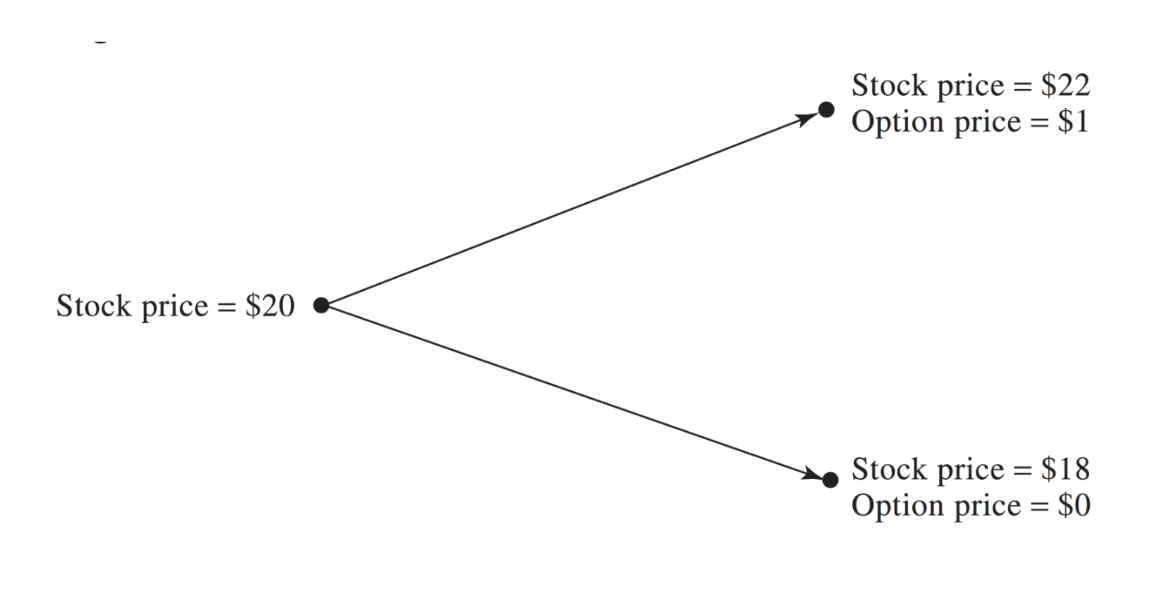
\includegraphics[scale=0.3]{tree-ex.png}
\end{figure}
\end{center}

To price the option, we will construct a portfolio consisting of the stock and the option in such a way that there is no uncertainty about the value of the portfolio at time $T$.  Then, we can argue that since the portfolio has no risk, the return it earns must equal the risk-free interest rate (otherwise, an arbitrage opportunity would exist).

Consider a portfolio consisting of a long position in $\Delta$ shares of the stock and a short position in one call option.  (We will determine the value of $\Delta$.)

\begin{ex}
Show that if $S_T=22$, then the total value of the portfolio at time $T$ is $22\Delta-1$.
\end{ex}

\begin{ex}
Show that if $S_T=18$, then the total value of the portfolio at time $T$ is $18\Delta$.
\end{ex}

\begin{df} The portfolio is {\bf riskless} if the final value is the same for both cases (i.e. both possible values of $S_T$).
\end{df}  

\begin{ex}
Find the value of $\Delta$ that makes this portfolio riskless, and conclude that, regardless of whether the stock price moves up or down, the value of the portfolio is always \$4.5 at time $T$.
\end{ex}



\begin{ex}
Suppose that the risk-free annual interest rate (compounded continuously) is 12\% and that $T=3$ months.  Show that the value of the portfolio today is \$4.367. 
\end{ex}

\begin{ex}
Show that, in the absence of arbitrage, the price of the call option today is \$0.633.
\end{ex}

\noindent In particular, it is important to observe that if the current value of the option were {\em not} \$0.633, then an arbitrage opportunity would exist.  If the value of the option were more than \$0.633, the portfolio would cost less than \$4.367 to set up and would earn more than the risk-free interest rate.  If the value of the option were less than \$0.633, an investor could short the portfolio to borrow money at less than the risk-free rate, and therefore earn a riskless profit.

\smallskip

We can generalize this no-arbitrage argument in the following way.  Consider a stock whose current price is $S_0$ and a European call option on the stock whose current price is $f$.  Suppose that $T$ is the maturity time of the option and that between the current time ($t=0$) and the expiry of the option ($t=T$), the stock price will either increase to $S_0u$, where $u>1$, or decrease to $S_0d$, where $d<1$.  Let $f_u$ denote the payoff from the option if $S_T=S_0u$, and let $f_d$ denote the payoff from the option if $S_T=S_0d$.  This is illustrated in the following figure.

\begin{center}
\begin{figure}[H]
\includegraphics[scale=0.3]{tree-general.png}
\end{figure}
\end{center}

As before, consider a portfolio consisting of a long position in $\Delta$ shares of the stock and a short position in one European call option on the stock.

\begin{ex}
Recall that the portfolio is riskless if the portfolio is worth the same amount at time $T$ in both cases (i.e. $S_T=S_0u$ or $S_T=S_0d$).  Find the value of $\Delta$ that makes the portfolio riskless.
\end{ex}

\begin{ex}\label{option-price}{\bf One-Step Binomial Tree Option Price}
Use the present value of the portfolio and the expression for $\Delta$ that you obtained in the previous exercise to show that $$f=e^{-rT}\left[pf_u+(1-p)f_d\right],$$ where $$p=\frac{e^{rT}-d}{u-d}.$$
\end{ex}


Observe that in using binomial trees to price options, no assumptions were required about the probabilities of up and down movements of the stock price at each node of the tree.  This is surprising and somewhat counterintuitive.  For example, we get the same option price when the probability of an upward movement is $0.5$ as we do when it is $0.9$. This is surprising and seems counterintuitive. It is natural to assume that, as the probability of an upward movement in the stock price increases, the value of a call option on the stock increases and the value of a put option on the stock decreases. This is not the case.  The key reason is that we are not valuing the option in absolute terms. We are calculating its value in terms of the price of the underlying stock. The probabilities of future up or down movements are already incorporated into the stock price: we do not need to take them into account again when valuing the option in terms of the stock price.

\begin{ex}
Use this expression for $f$ to show that $f=\$0.633$ for the numerical example considered previously in this section.
\end{ex}

\begin{ex}
A stock price is currently \$100. Over each of the next two 6-month periods it is expected to go up by 10\% or down by 10\%. The risk-free interest rate is 8\% per annum with continuous compounding. What is the value of a 1-year European call option with a strike price of \$100?
\end{ex}

\begin{ex}
For the situation considered in the previous exercise, what is the value of a 1-year European put option with a strike price of \$100? 
\end{ex}



\begin{ex}
A stock price is currently \$25. It is known that at the end of 2 months it will be either \$23 or \$27. The risk-free interest rate is 10\% per annum with continuous compounding. Suppose $S_T$ is the stock price at the end of 2 months. What is the value of a derivative that pays $S_T^2$ at this time?
\end{ex}

\bigskip

\hrule

\bigskip

\subsection{Two-Step Binomial Trees}


\begin{ex}{\bf Two-Step Binomial Tree Option Price}
Consider a stock whose current price is $S_0$ and a European call option on the stock whose current price is $f$.  Suppose that there are two time steps, each of length $\Delta t$, before expiry, and that during each time step, the stock price either moves up to $u$ times its initial value ($u>1$) or down to $d$ times its initial value ($d<1$).  This is illustrated in the following figure, using the same notation as in the previous figure for the payoff from the option at each stage.  (For example, $f_{uu}$ is the value of the option at time $2\Delta t=T$ if $S_T=u^2S_0$, i.e. if the stock increases in value at each time step.

\begin{center}
\begin{figure}[H]
\includegraphics[scale=0.3]{two-step-tree.png}
\end{figure}
\end{center}

Show that $$f=e^{-2r\Delta t}\left[p^2f_{uu}+2p(1-p)f_{ud}+(1-p)^2f_{dd}\right].$$

\end{ex}


\begin{ex}
A stock price is currently \$50. Over each of the next two 3-month periods it is expected to go up by 6\% or down by 5\%. The risk-free interest rate is 5\% per annum with continuous compounding. What is the value of a 6-month European call option with a strike price of \$51?
\end{ex}



Clearly, an analyst can expect to obtain only a very rough approximation to an option price by assuming that stock price movements during the life of the option consist of one or two binomial steps. When binomial trees are used in practice, the life of the option is typically divided into $30$ or more time steps, and at each time step, there is a binomial stock price moment.  Although the mathematical methods are exactly the same as those presented here, the number of computations that must be performed becomes extremely large (and requires the use of powerful computing software).  For example, with $30$ time steps, there are $31$ possibilities for the terminal stock price and $2^{30}$, or about $1$ billion, possible paths in the binomial tree.

\bigskip

\hrule

\bigskip

\subsection{Delta}

\begin{df}{\bf Delta}
The {\bf delta} of a stock option is the ratio of the change in the price of the stock option to the change in the price of the underlying stock.  It is the number of units of the stock we should hold for each option shorted in order to create a riskless portfolio.  
\end{df}

\begin{itemize}

\item The construction of a riskless portfolio is referred to as {\em delta hedging}.

\item The delta of a call option is positive.

\item The delta of a put option is positive.

\item Note that delta changes over time.

\end{itemize}

\noindent 





 
\end{document}